\documentclass[journal]{IEEEtran}
\usepackage[a5paper, margin=10mm]{geometry}
%\usepackage{lmodern} % Ensure lmodern is loaded for pdflatex
\usepackage{tfrupee} % Include tfrupee package

\setlength{\headheight}{1cm}
\setlength{\headsep}{0mm}

\usepackage{gvv-book}
\usepackage{gvv}
\usetikzlibrary{patterns}
\lstset{aboveskip=12pt}
\usepackage[center]{caption}
\raggedbottom

\hypersetup{
    colorlinks=true,
    urlcolor=black
}
\usepackage{amsfonts}
\makeindex

\begin{document}
\bibliographystyle{IEEEtran}
\onecolumn

\title{
    \begin{center}
        Math for EE
        \\
        \rule{0.4\columnwidth}{0.4pt}
    \end{center}
}
\author{
    \vspace{11cm}
    \begin{center}
        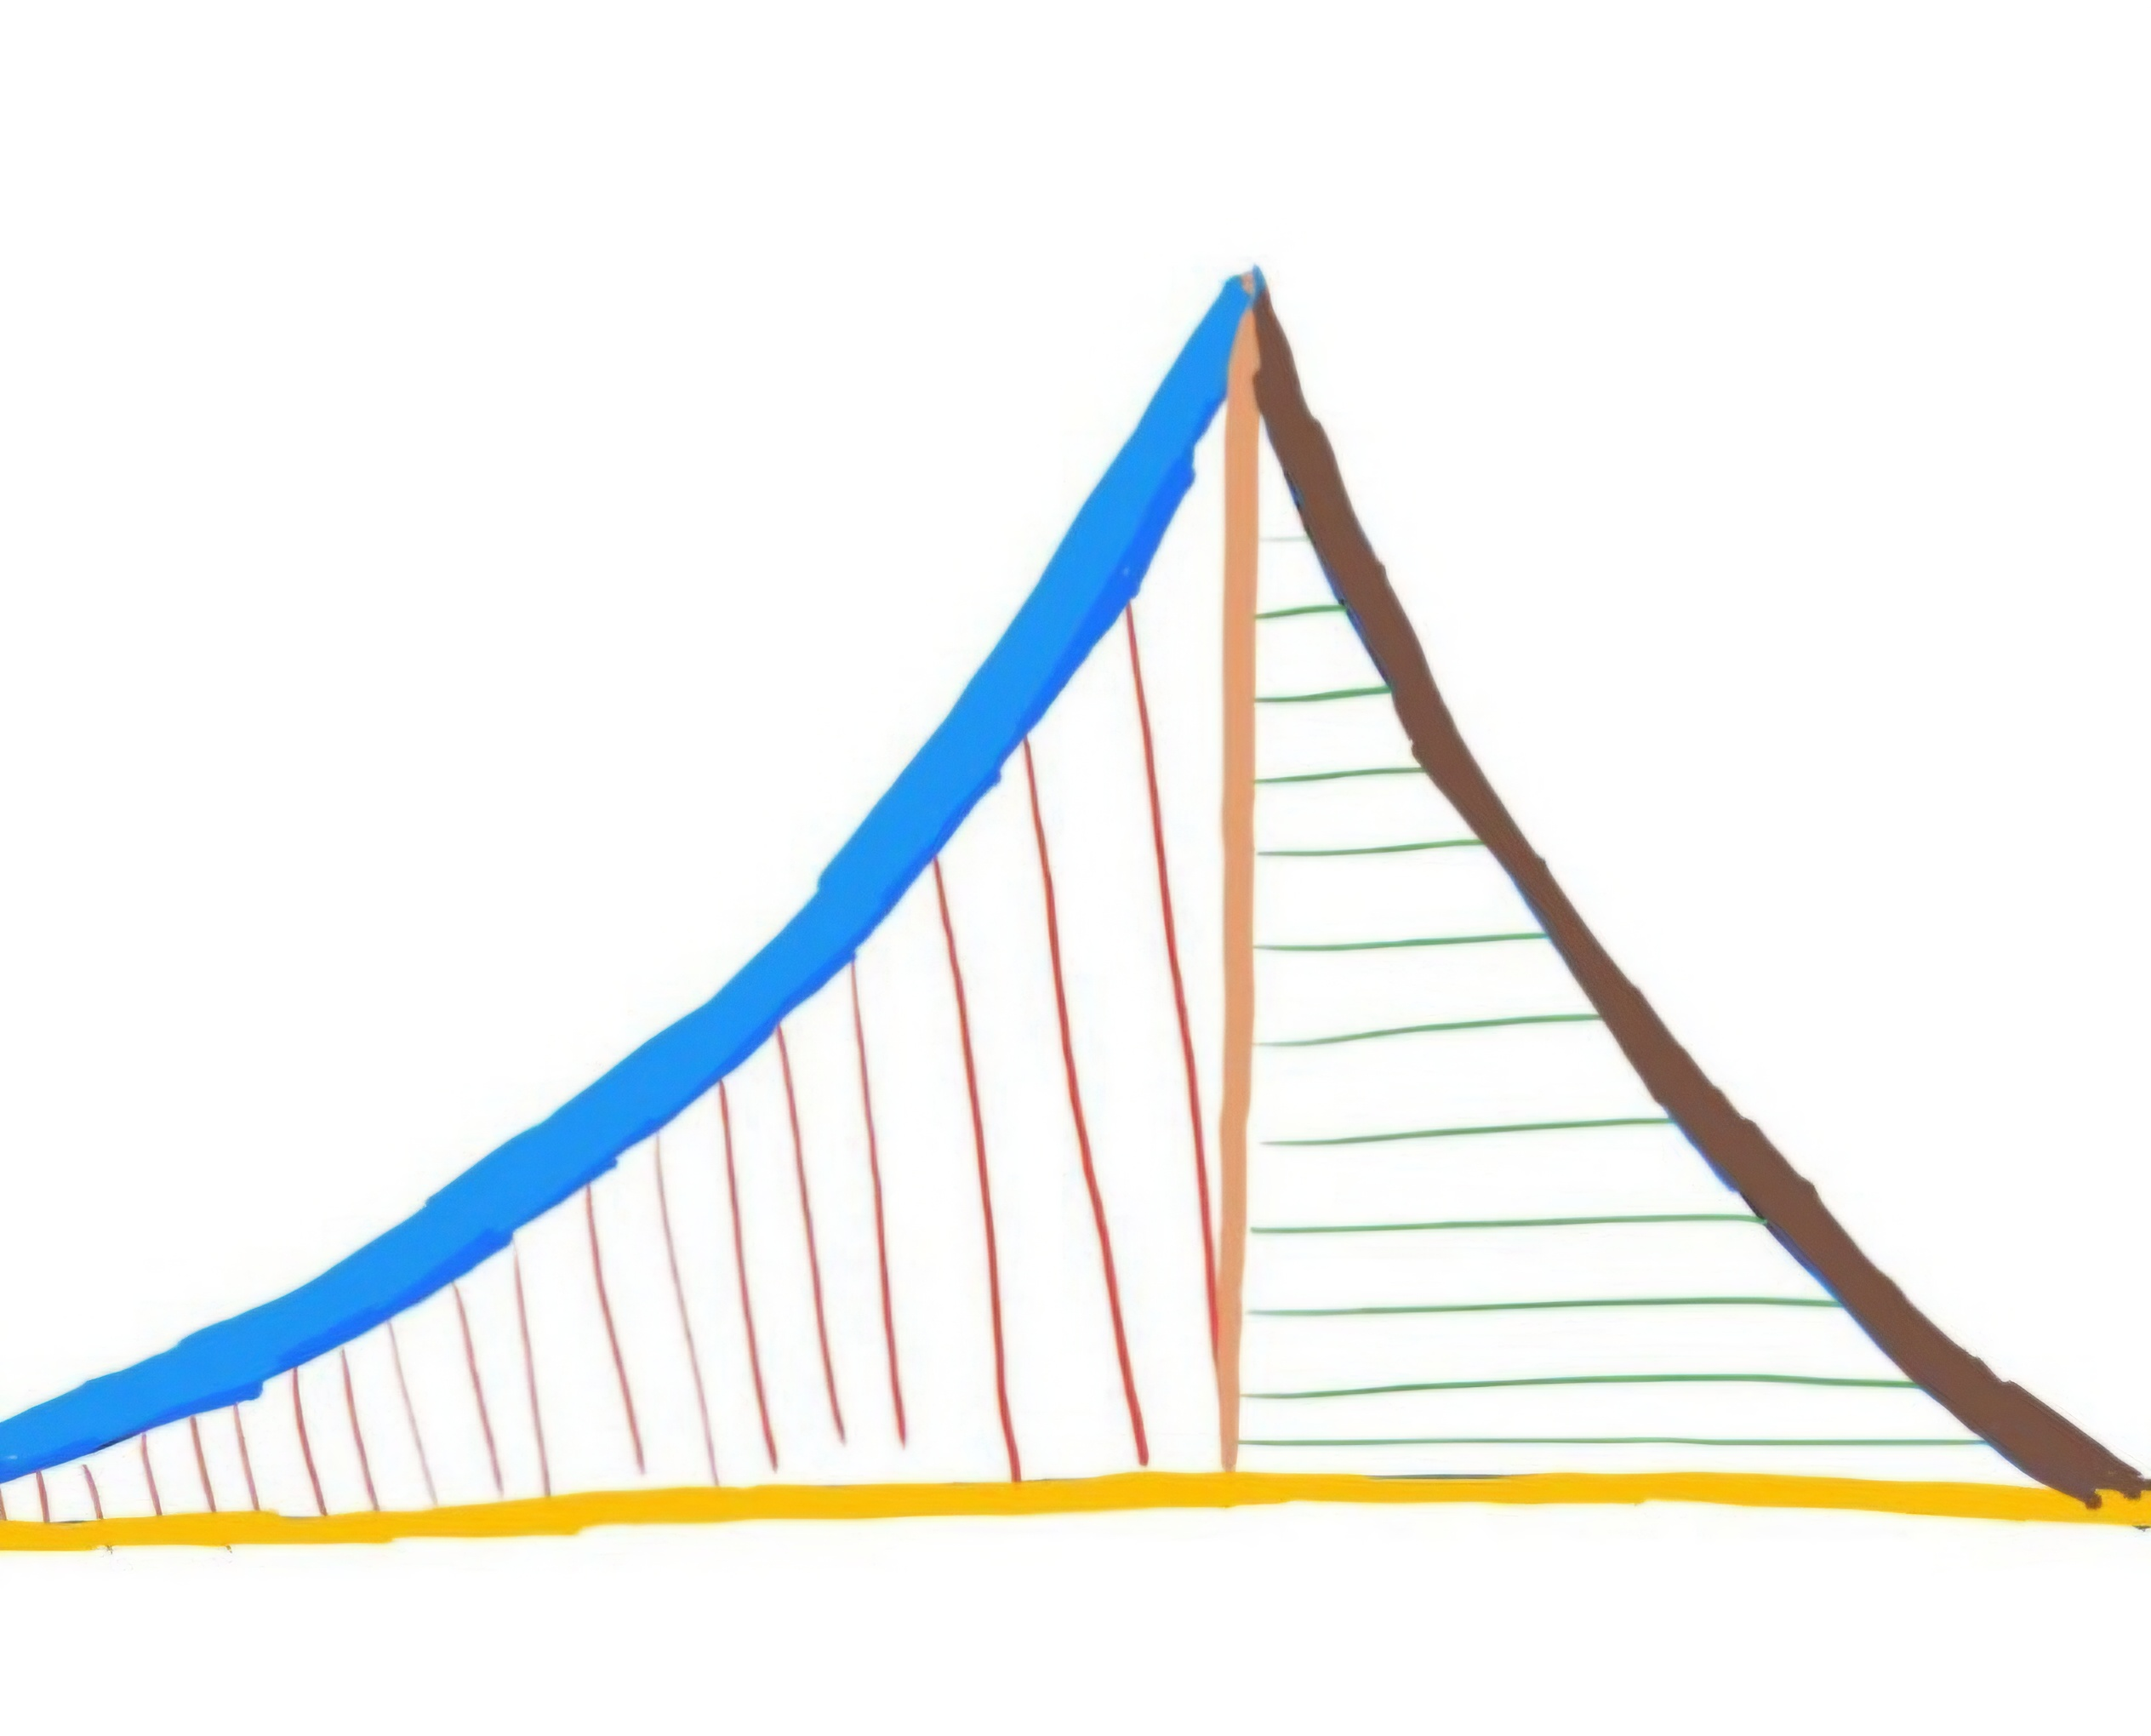
\includegraphics[width=0.2\columnwidth]{figs/logo.jpg}
        \\
        {\huge G. V. V. Sharma}
    \end{center}
}
\maketitle

\newpage
\section*{About this Book}

This book introduces matrices through high school coordinate geometry.
This approach makes it easier for beginners to learn Python for scientific
computing. All problems in the book are from NCERT mathematics textbooks
from Class 9--12. Exercises are from CBSE board exam papers.

The content is sufficient for industry jobs and covers nearly all matrix
prerequisites for machine learning. There is no copyright, so readers are
free to print and share.
License: https://creativecommons.org/licenses/by-sa/3.0/
\\
and
\\
https://www.gnu.org/licenses/fdl-1.3.en.html
\\
First manual appeared in January 2018
\\
First edition published on July 10, 2024
\\
In this edition, some incorrect solutions were removed. All figures
redrawn. More problems added.

\newpage
\onecolumn
\begin{center}
{\Large\bfseries CBSE 2026 12th class maths solutions (65-5-1)}
\end{center}
\vspace{0.4em}

\begin{list}{}{\setlength{\leftmargin}{1.15cm}\setlength{\labelwidth}{1.0cm}\setlength{\labelsep}{0.15cm}\setlength{\itemindent}{0pt}\setlength{\listparindent}{0pt}\setlength{\itemsep}{\baselineskip}\setlength{\parsep}{0pt}\setlength{\topsep}{0pt}}
\item[5.1.1] If matrix $A=\begin{bmatrix}-p&q\\r&p\end{bmatrix}$ is such that $A^2=I$, then:

\noindent (A) $1+p^2+qr=0$ \hfill (B) $1-p^2-qr=0$ \\
(C) $1-p^2+qr=0$ \hfill (D) $1+p^2-qr=0$

\vspace{0.6em}\par\noindent\textbf{Solution:}

Squaring the matrix gives
\[
A^2=\begin{bmatrix}p^2+qr&0\\0&p^2+qr\end{bmatrix}=(p^2+qr)I.
\]
Since $A^2=I$, we have $p^2+qr=1$, or $1-p^2-qr=0$. The correct answer is \textbf{(B)}.

\item[5.1.2] If $A$ is a square matrix such that $A^2=A$, then $(A-I)^3-A$ is equal to:

\noindent (A) $I$ \hfill (B) $-I$ \hfill (C) $A$ \hfill (D) $A^2$

\vspace{0.6em}\par\noindent\textbf{Solution:}

Using $A^2=A$,
\[
(A-I)^2=A^2-2A+I=I-A,
\]
and hence
\[
(A-I)^3=(I-A)(A-I)=A-I.
\]
Therefore $(A-I)^3-A=(A-I)-A=-I$. The correct answer is \textbf{(B)}.

\item[5.1.4] Let
\[
A=\begin{bmatrix}0&-3&4\\1&0&2\end{bmatrix},\qquad
B=\begin{bmatrix}-3&0&1\\2&4&0\end{bmatrix}.
\]
If $A+B+C=O$, then matrix $C$ is:

\noindent (A) $\begin{bmatrix}-3&-3&5\\3&4&2\end{bmatrix}$ \hfill
(B) $\begin{bmatrix}3&3&5\\-3&-4&-2\end{bmatrix}$ \\
(C) $\begin{bmatrix}3&3&-5\\-3&-4&-2\end{bmatrix}$ \hfill
(D) $\begin{bmatrix}-3&-3&-5\\3&4&2\end{bmatrix}$

\vspace{0.6em}\par\noindent\textbf{Solution:}

$C=-(A+B)$. Adding the matrices gives $A+B=\begin{bmatrix}-3&-3&5\\3&4&2\end{bmatrix}$, so
\[
C=\begin{bmatrix}3&3&-5\\-3&-4&-2\end{bmatrix}.
\]
The answer is \textbf{(C)}.

\item[5.1.5] If $A$ is a non-singular matrix, which statement is not true?

\noindent (A) $\operatorname{adj} A$ is singular \hfill
(B) $(\operatorname{adj} A)^{-1}=\operatorname{adj}(A^{-1})$ \\
(C) $|A|\ne0$ \hfill (D) $A^{-1}$ exists

\vspace{0.6em}\par\noindent\textbf{Solution:}

For a non-singular matrix, $|A|\ne0$ and $A^{-1}$ exists. Also $\operatorname{adj}A=|A|A^{-1}$ is non-singular. Therefore the false statement is that $\operatorname{adj}A$ is singular, option \textbf{(A)}. The accompanying plot uses a sample matrix family to illustrate that singularity occurs only when its determinant is zero.
\begin{lstlisting}[frame=single, basicstyle=\rmfamily, escapeinside={(*@}{@*)}]
(*@\makebox[\dimexpr\linewidth-2\fboxsep-2\fboxrule\relax][c]{codes/5.1.5.py}@*)
\end{lstlisting}
\begin{figure}[H]
\centering
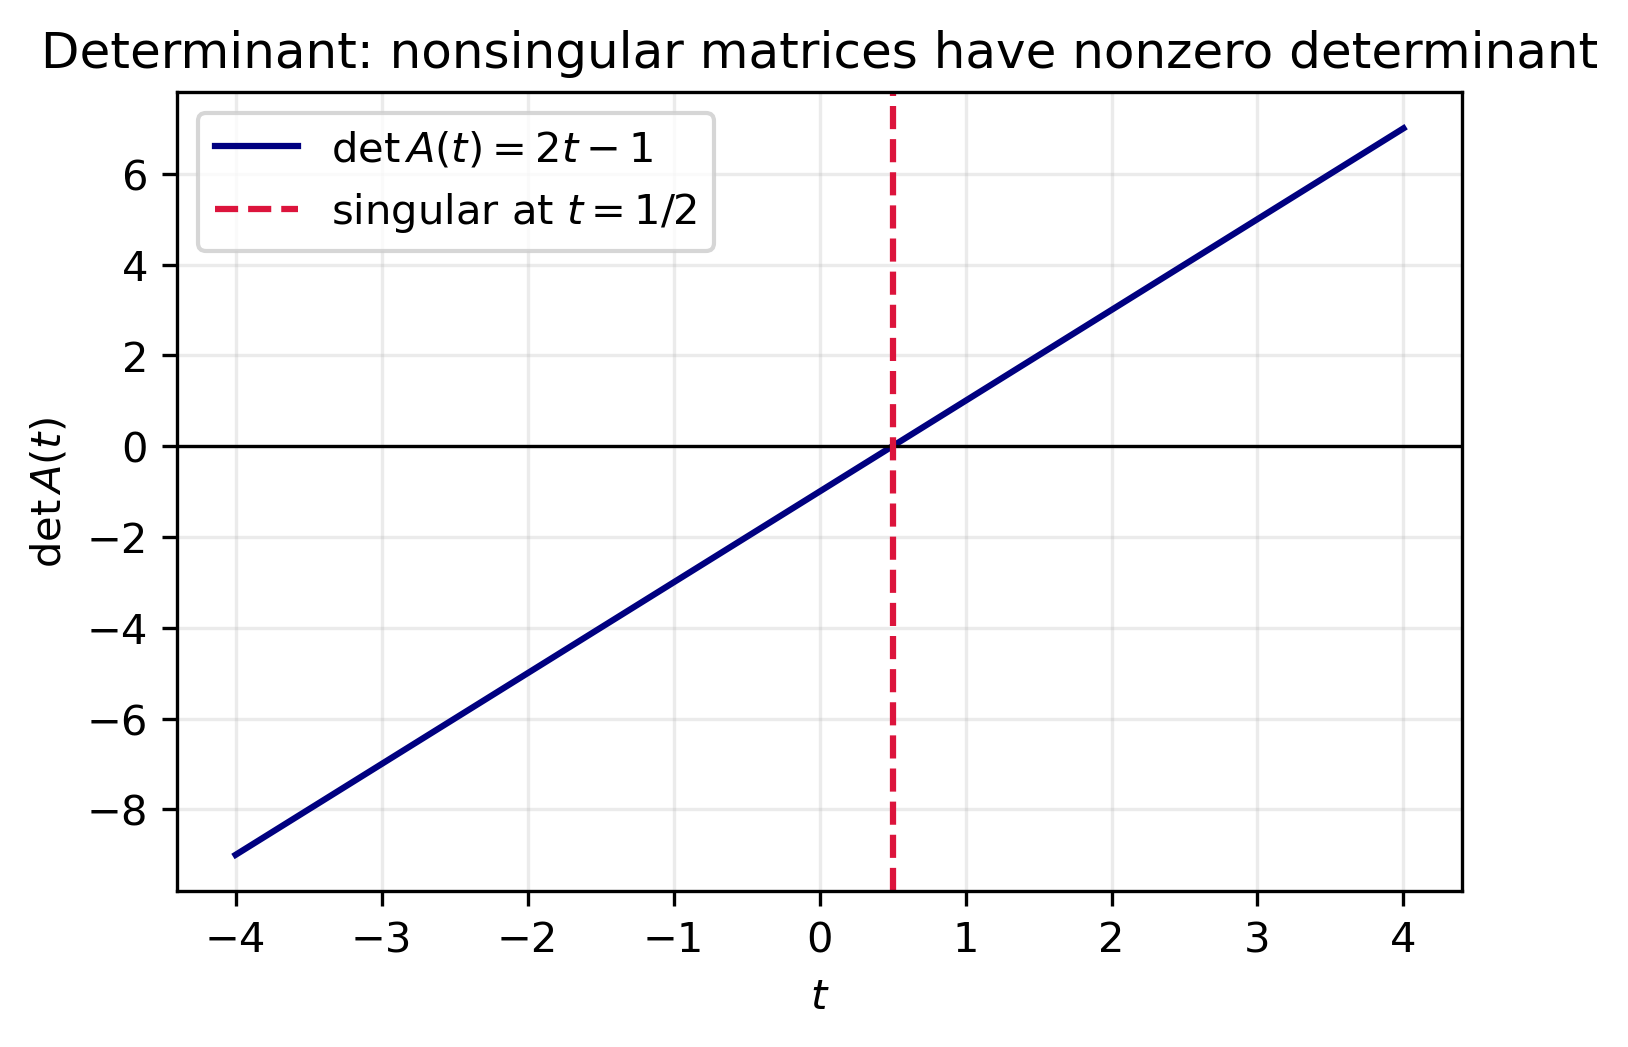
\includegraphics[width=0.48\linewidth]{figs/5.1.5.png}
\caption{Determinant of a representative matrix family.}
\end{figure}

\item[5.1.6] If
\[
f(x)=\begin{cases}\dfrac{x^2-4x-5}{x+1},&x\ne-1,\\ k,&x=-1,\end{cases}
\]
is continuous at $x=-1$, find $k$.

\vspace{0.6em}\par\noindent\textbf{Solution:}

For $x\ne-1$, $f(x)=\frac{(x-5)(x+1)}{x+1}=x-5$. Thus $\lim_{x\to-1}f(x)=-6$, and continuity requires $k=-6$, option \textbf{(D)}. The code plots the resulting continuous function.
\begin{lstlisting}[frame=single, basicstyle=\rmfamily, escapeinside={(*@}{@*)}]
(*@\makebox[\dimexpr\linewidth-2\fboxsep-2\fboxrule\relax][c]{codes/5.1.6.py}@*)
\end{lstlisting}
\begin{figure}[H]
\centering
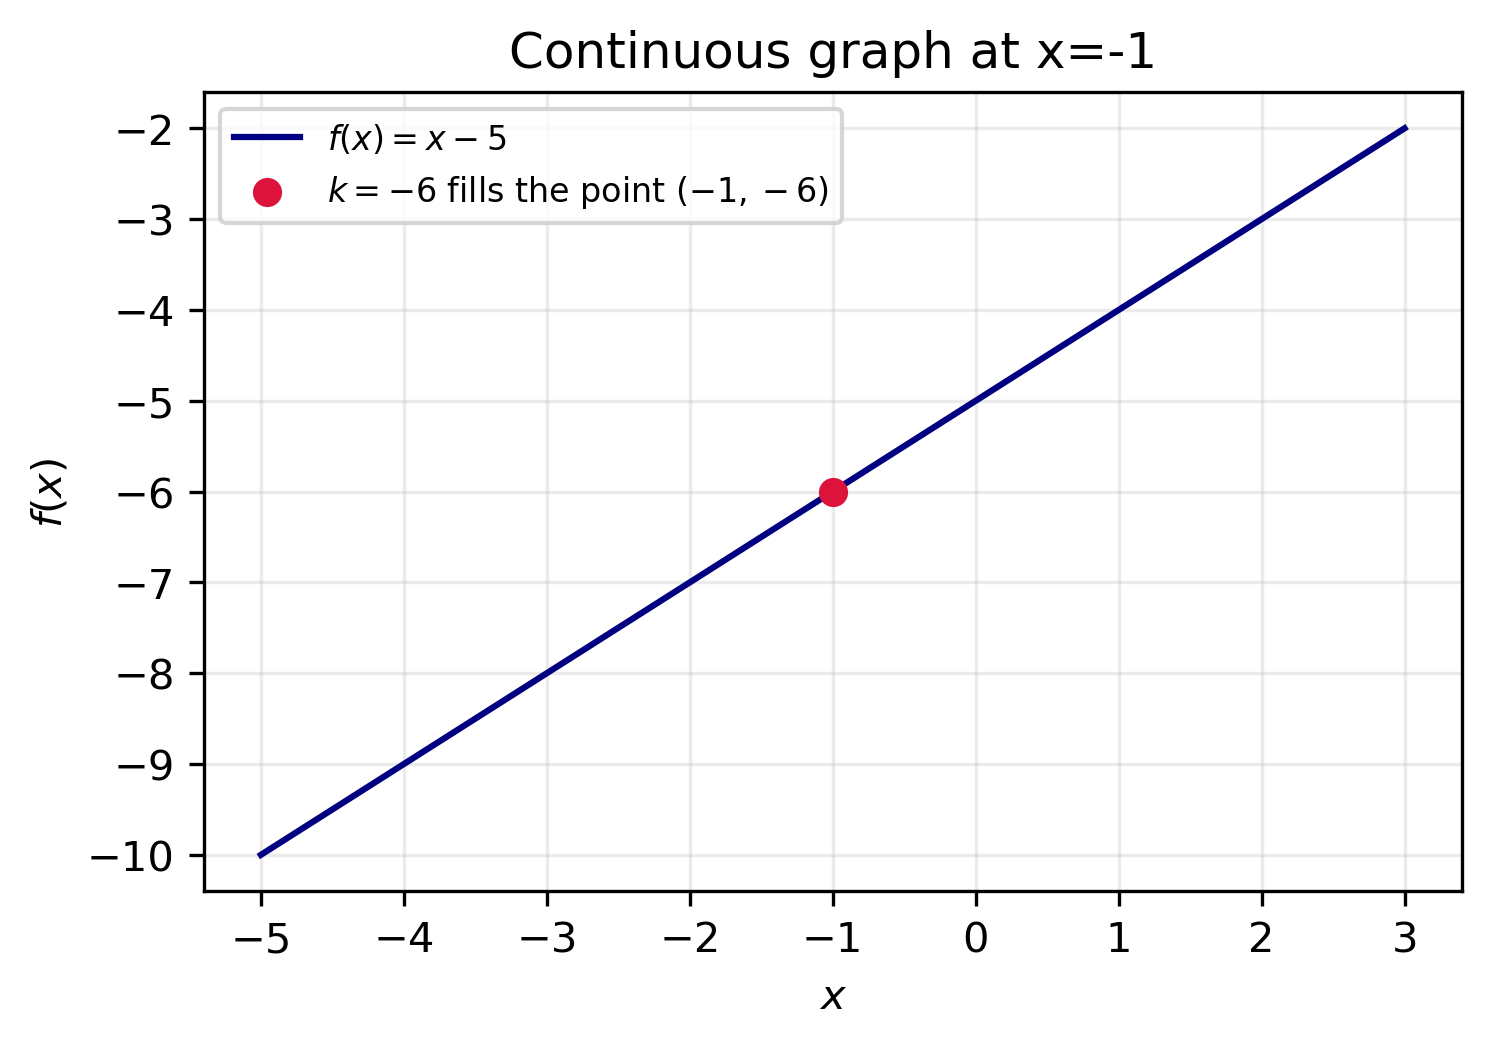
\includegraphics[width=0.47\linewidth]{figs/5.1.6.png}
\caption{The continuous extension at $x=-1$.}
\end{figure}

\item[5.1.7] The triangle with vertices $A(3,1)$, $B(-2,1)$ and $C(0,k)$ has area $5$ square units. Find $k$.

\noindent (A) $3,1$ \hfill (B) $-1,3$ \hfill (C) $-1,2$ \hfill (D) $0,2$

\vspace{0.6em}\par\noindent\textbf{Solution:}

The base $AB$ has length $5$ and the perpendicular height is $|k-1|$. Hence $\frac12(5)|k-1|=5$, giving $|k-1|=2$, so $k=-1$ or $k=3$, option \textbf{(B)}. Both triangles are plotted by the code.
\begin{lstlisting}[frame=single, basicstyle=\rmfamily, escapeinside={(*@}{@*)}]
(*@\makebox[\dimexpr\linewidth-2\fboxsep-2\fboxrule\relax][c]{codes/5.1.7.py}@*)
\end{lstlisting}
\begin{figure}[H]
\centering
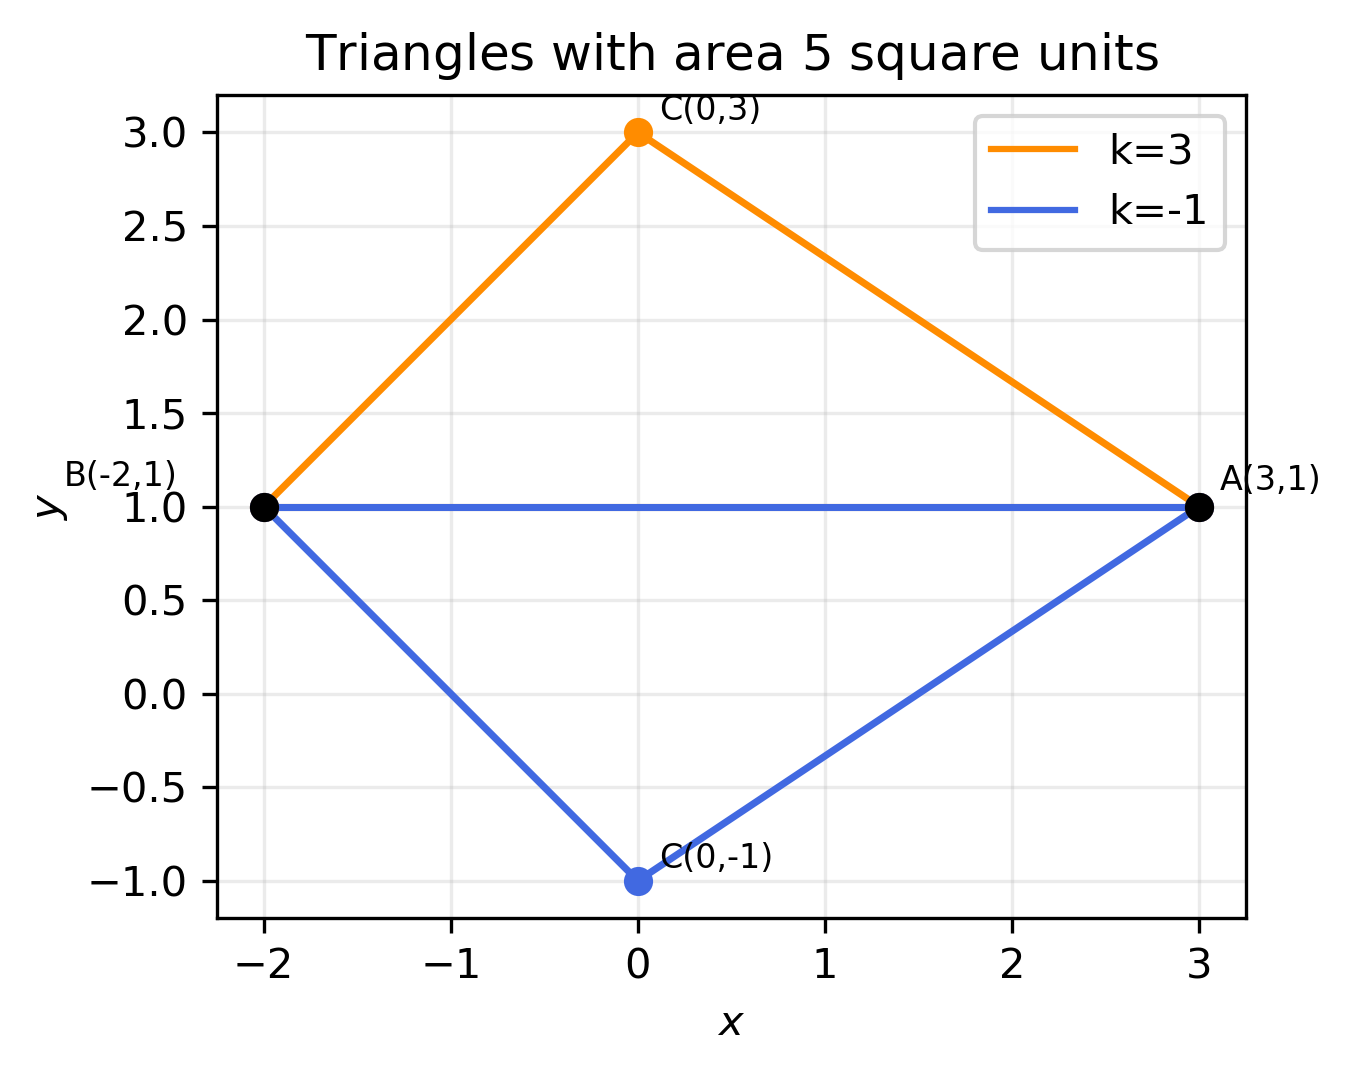
\includegraphics[width=0.48\linewidth]{figs/5.1.7.png}
\caption{Both possible triangles with area $5$.}
\end{figure}

\item[5.1.9] Find the absolute minimum value of $f(x)=(x-2)^2+5$ on $[-3,2]$.

\noindent (A) $-3$ \hfill (B) $2$ \hfill (C) $5$ \hfill (D) $30$

\vspace{0.6em}\par\noindent\textbf{Solution:}

Since $(x-2)^2\ge0$ with equality at the included endpoint $x=2$, the absolute minimum is $f(2)=5$, option \textbf{(C)}. The code performs a bounded numerical minimization and plots the function.
\begin{lstlisting}[frame=single, basicstyle=\rmfamily, escapeinside={(*@}{@*)}]
(*@\makebox[\dimexpr\linewidth-2\fboxsep-2\fboxrule\relax][c]{codes/5.1.9.py}@*)
\end{lstlisting}
\begin{figure}[H]
\centering
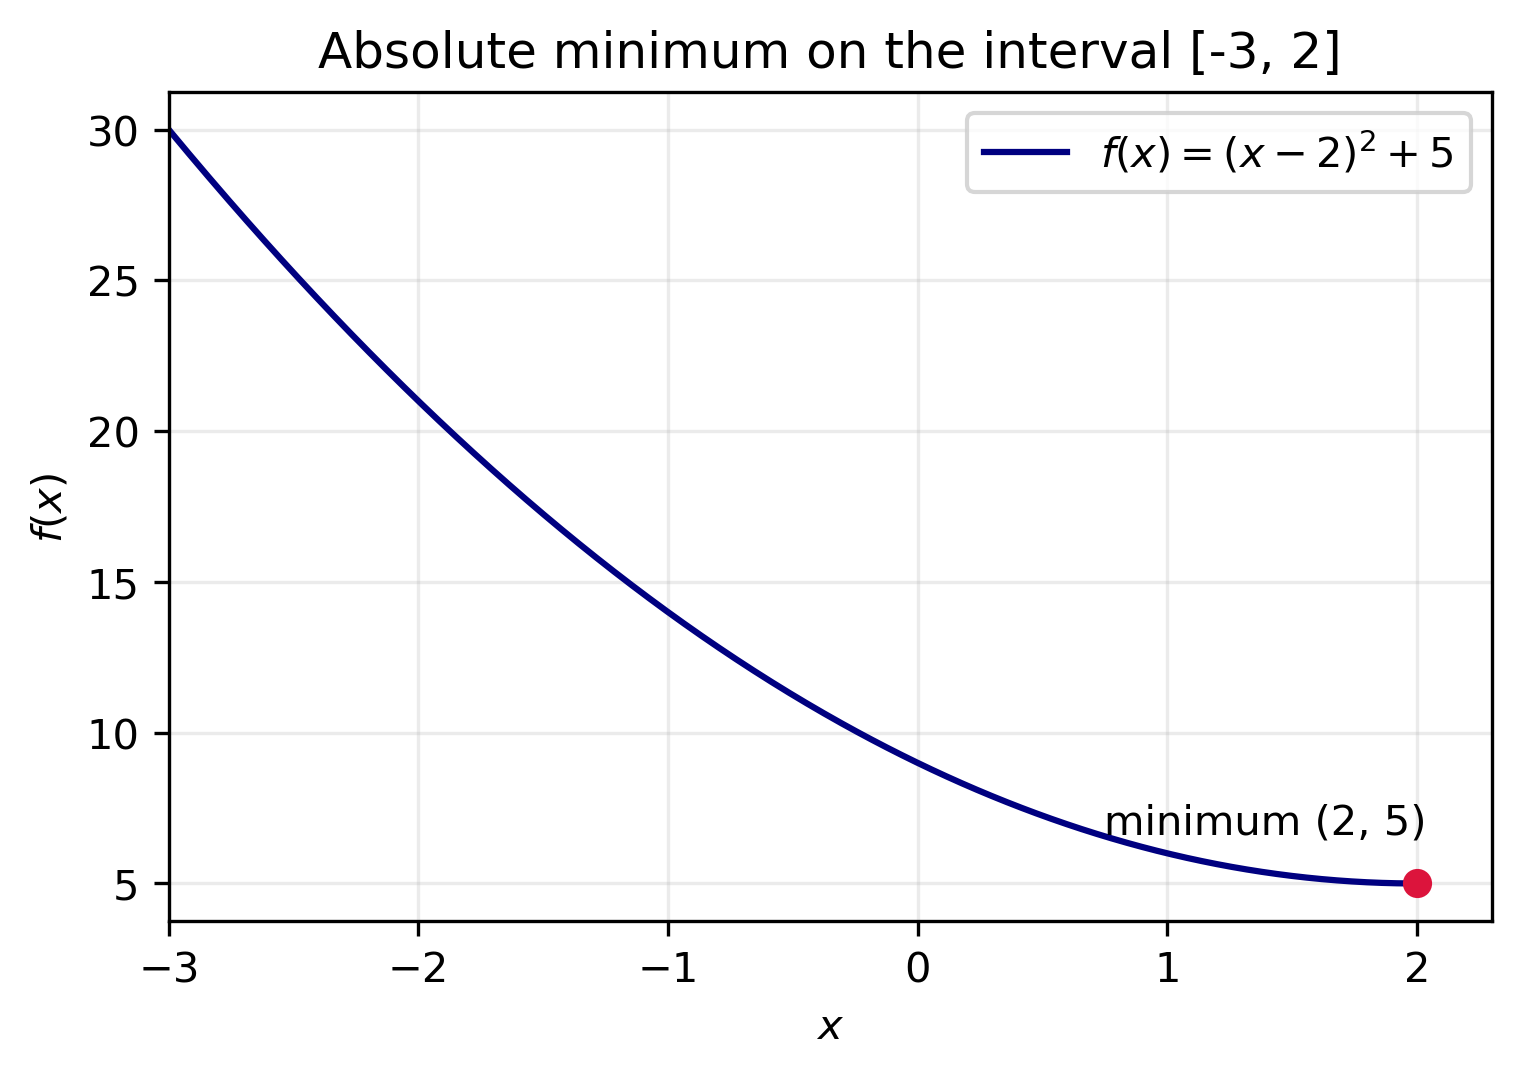
\includegraphics[width=0.48\linewidth]{figs/5.1.9.png}
\caption{The minimum occurs at $x=2$.}
\end{figure}

\item[5.1.10] Evaluate $\displaystyle\int\frac{1}{\sqrt{1+\cos2x}}\,dx$.

\noindent (A) $\log\cos x+C$ \hfill (B) $\frac1{\sqrt2}\log|\sec x+\tan x|+C$ \\
(C) $\frac1{\sqrt2}\log|\sec x-\tan x|+C$ \hfill (D) $\log\sin2x+C$

\vspace{0.6em}\par\noindent\textbf{Solution:}

Using $1+\cos2x=2\cos^2x$, the integrand is $\frac1{\sqrt2}\sec x$ on intervals where $\cos x>0$. Therefore
\[
\int\frac{dx}{\sqrt{1+\cos2x}}=\frac1{\sqrt2}\log|\sec x+\tan x|+C,
\]
which is option \textbf{(B)}.

\item[5.1.12] An ant crawls along the line $y=2x-4$. Find the area bounded by this line, the $y$-axis, the $x$-axis, and $x=1$.

\noindent (A) $1$ sq. unit \hfill (B) $3$ sq. units \\
(C) $2$ sq. units \hfill (D) $4$ sq. units

\vspace{0.6em}\par\noindent\textbf{Solution:}

For $0\le x\le1$, the line is below the $x$-axis, so the area is $\int_0^1(4-2x)\,dx=3$ square units, option \textbf{(B)}. The code plots the line and bounded region.
\begin{lstlisting}[frame=single, basicstyle=\rmfamily, escapeinside={(*@}{@*)}]
(*@\makebox[\dimexpr\linewidth-2\fboxsep-2\fboxrule\relax][c]{codes/5.1.12.py}@*)
\end{lstlisting}
\begin{figure}[H]
\centering
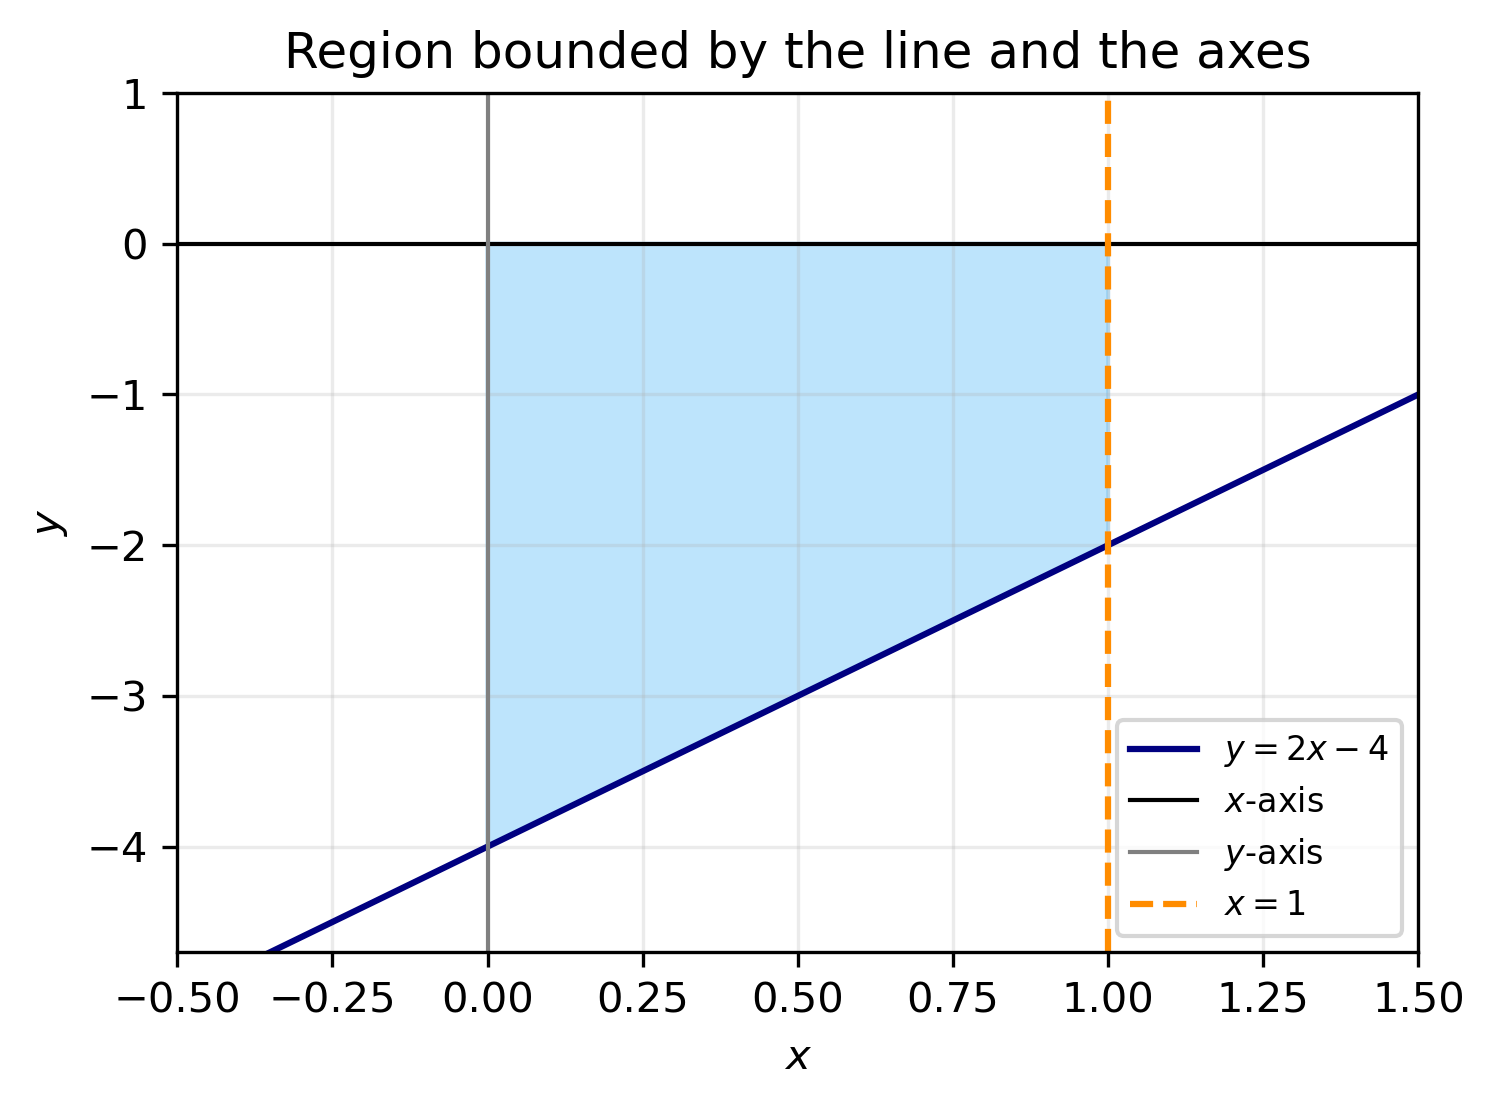
\includegraphics[width=0.46\linewidth]{figs/5.1.12.png}
\caption{Area enclosed by $y=2x-4$, the axes, and $x=1$.}
\end{figure}

\item[5.1.15] The feasible-region corner points are $(0,0),(0,40),(20,40),(60,20),(60,0)$. For $Z=4x+3y$, find the maximum value.

\noindent (A) $200$ \hfill (B) $300$ \hfill (C) $240$ \hfill (D) $120$

\vspace{0.6em}\par\noindent\textbf{Solution:}

At the listed corners, $Z$ takes values $0,120,200,300,240$, respectively. Thus the maximum is $300$ at $(60,20)$, option \textbf{(B)}. The code plots the feasible polygon and labels its corner values.
\begin{lstlisting}[frame=single, basicstyle=\rmfamily, escapeinside={(*@}{@*)}]
(*@\makebox[\dimexpr\linewidth-2\fboxsep-2\fboxrule\relax][c]{codes/5.1.15.py}@*)
\end{lstlisting}
\begin{figure}[H]
\centering
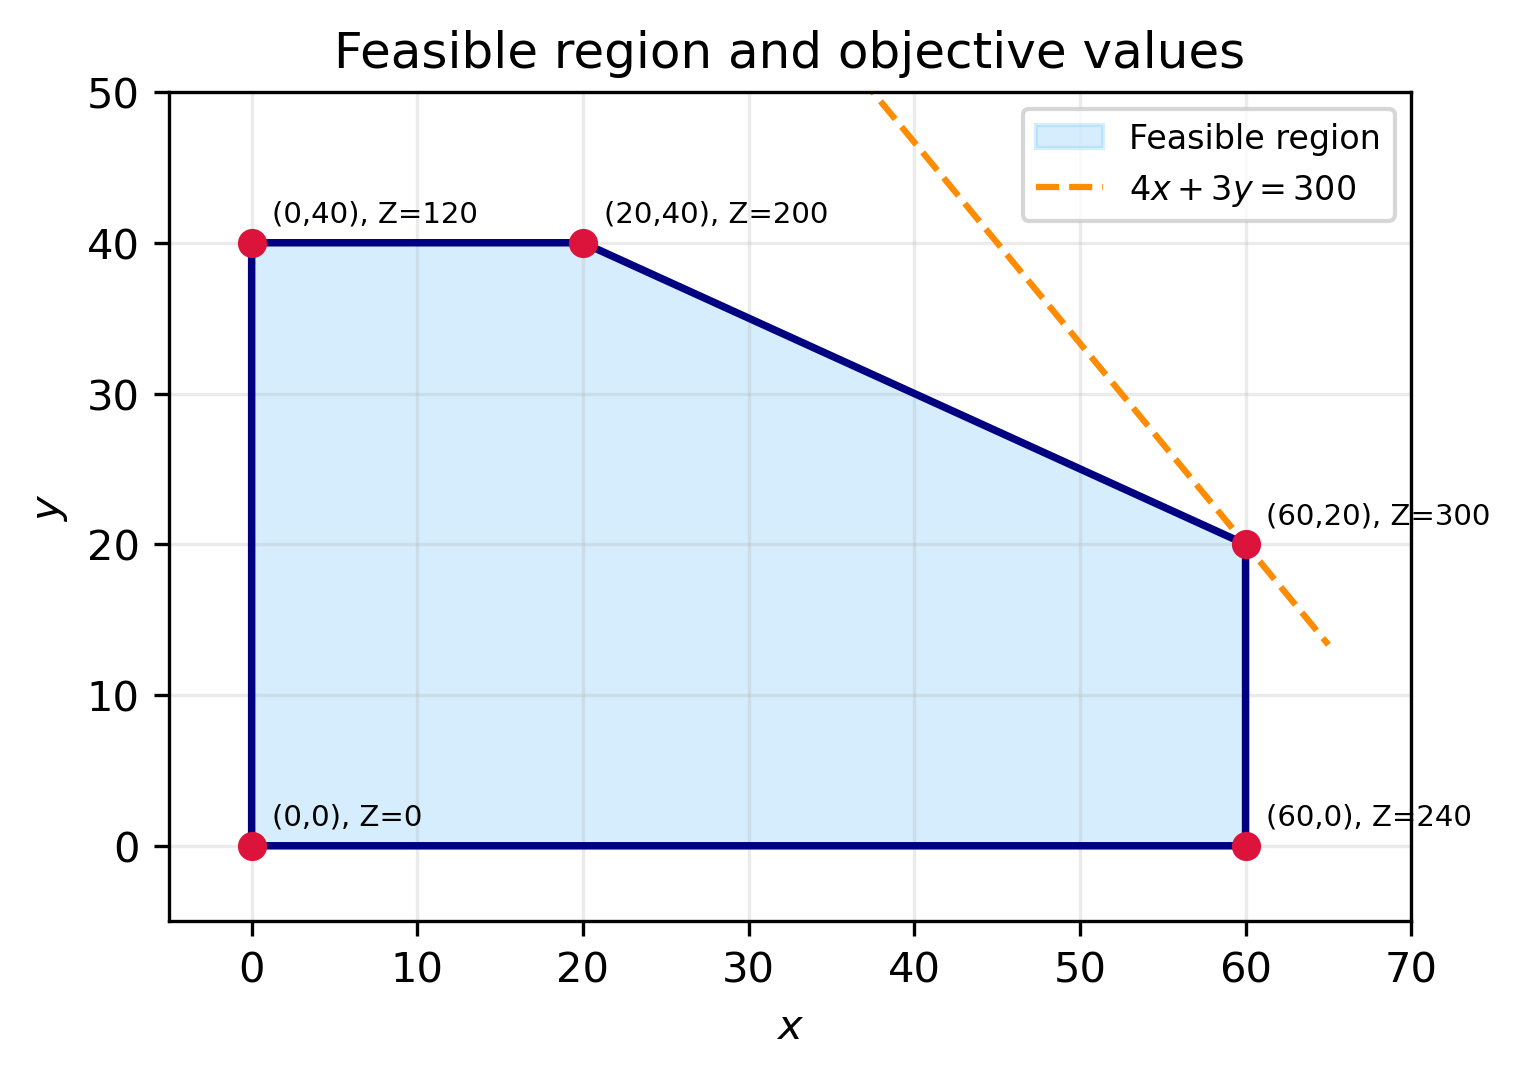
\includegraphics[width=0.52\linewidth]{figs/5.1.15.png}
\caption{Feasible region and objective values at its corners.}
\end{figure}

\item[5.1.18] Given $3P(A)=P(B)=\frac35$ and $P(A\mid B)=\frac23$, find $P(A\cup B)$.

\noindent (A) $\frac35$ \hfill (B) $\frac15$ \hfill (C) $\frac{2}{15}$ \hfill (D) $\frac25$

\vspace{0.6em}\par\noindent\textbf{Solution:}

As printed, $P(A)=\frac15$ and $P(B)=\frac35$. The conditional probability gives $P(A\cap B)=P(A\mid B)P(B)=\frac25$, so direct substitution into the union formula yields $P(A\cup B)=\frac15+\frac35-\frac25=\frac25$ (option \textbf{(D)}). However, these data are inconsistent: an intersection cannot have probability $\frac25$ when $P(A)=\frac15$. Thus option (D) is the formal calculation from the printed values, but the question appears to contain a typo.

\item[5.1.20] Consider minimizing $Z=x+2y$ subject to $2x+y\ge3$, $x+2y\ge6$, and $x,y\ge0$. The assertion says the minimum occurs at infinitely many points and the feasible-region corners are $(0,3)$ and $(6,0)$. The reason says that if two corners give the same minimum, every point on the segment between them also gives that minimum. Select the correct assertion-reason choice.

\vspace{0.6em}\par\noindent\textbf{Solution:}

The two corners both give $Z=6$. Since $Z$ is linear, every point on the segment joining them also gives $Z=6$, and the constraints are satisfied along that segment. Both statements are true, and the reason explains the assertion: option \textbf{(A)}. The code plots the constraint boundaries and the optimal segment.
\begin{lstlisting}[frame=single, basicstyle=\rmfamily, escapeinside={(*@}{@*)}]
(*@\makebox[\dimexpr\linewidth-2\fboxsep-2\fboxrule\relax][c]{codes/5.1.20.py}@*)
\end{lstlisting}
\begin{figure}[H]
\centering
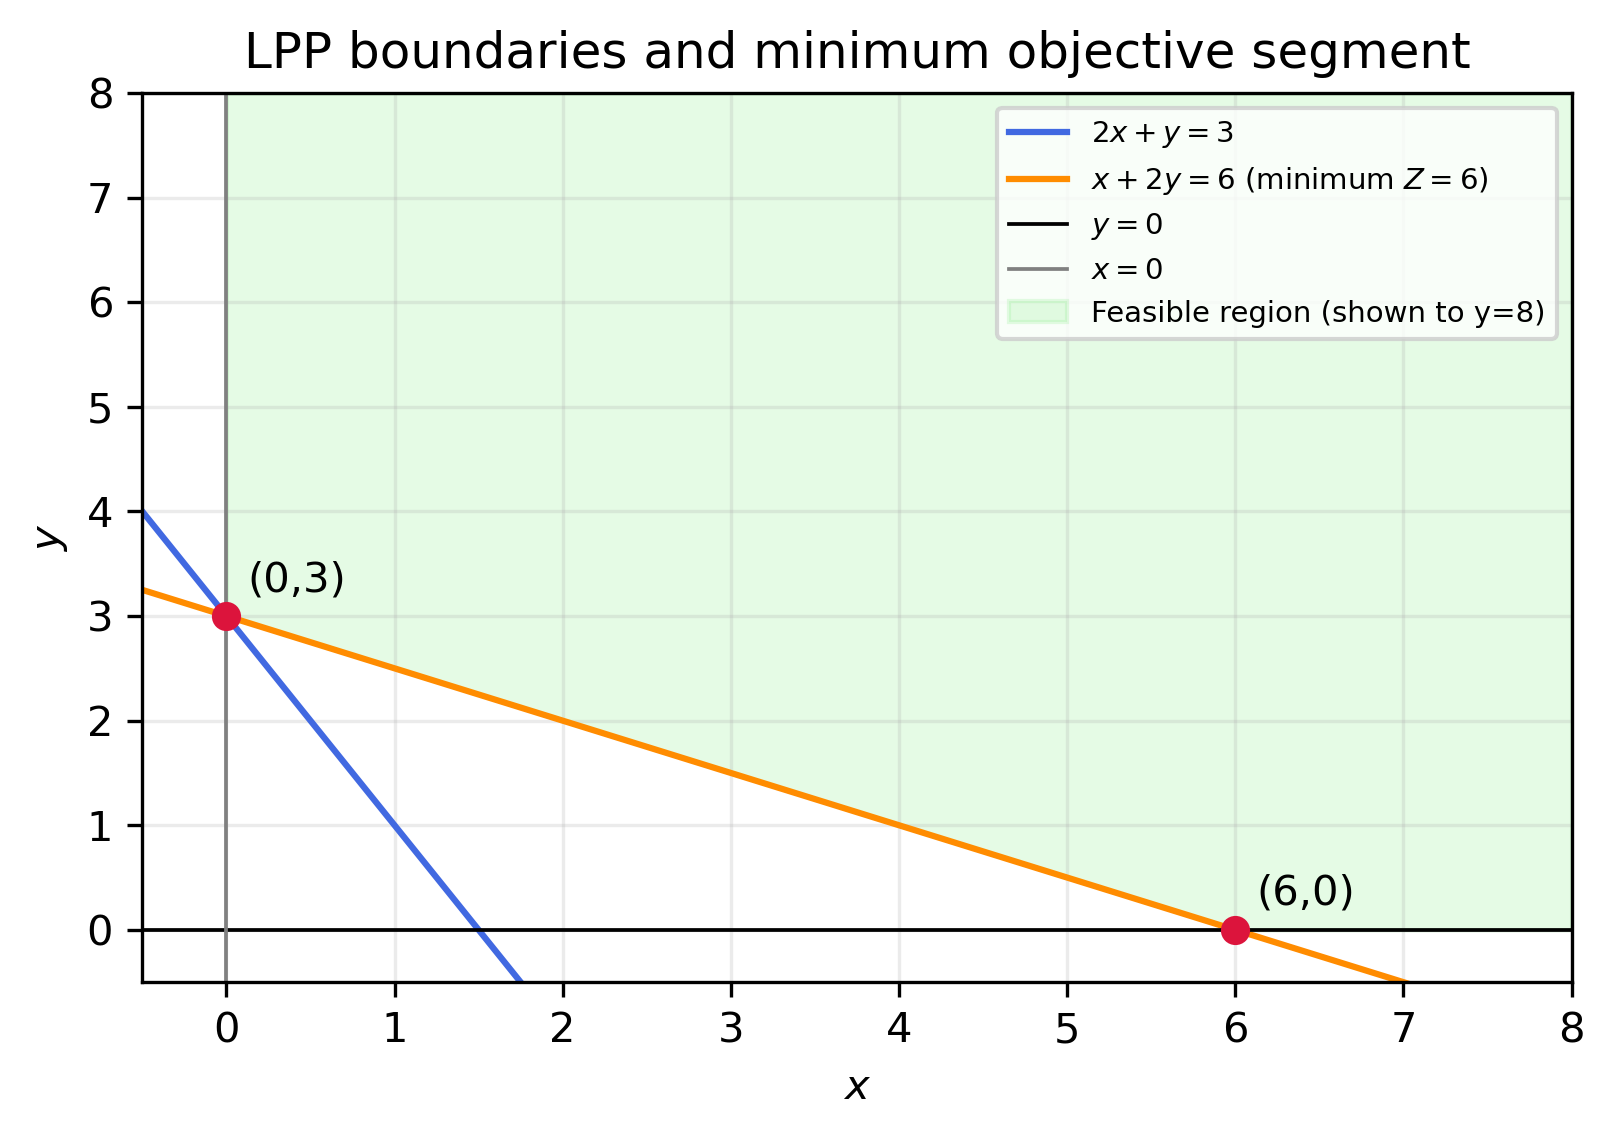
\includegraphics[width=0.52\linewidth]{figs/5.1.20.png}
\caption{Constraints and the segment of optimal points.}
\end{figure}

\item[5.1.22.1] Differentiate $x^x$ with respect to $x\log x$.

\vspace{0.6em}\par\noindent\textbf{Solution:}

Let $t=x\log x$ and $y=x^x$. Then $\log y=x\log x=t$, so $y=e^t$. Hence $\frac{dy}{d(x\log x)}=\frac{dy}{dt}=e^t=x^x$.

\item[5.1.22.2] If $y=P\cos ux+Q\sin ux$, show that $\frac{d^2y}{dx^2}+u^2y=0$.

\vspace{0.6em}\par\noindent\textbf{Solution:}

Differentiating twice gives $y''=-Pu^2\cos ux-Qu^2\sin ux=-u^2y$. Therefore $y''+u^2y=0$.

\item[5.1.23] Find the values of $x$ for which $f(x)=\frac{x-3}{x+1}$, $x\ne-1$, is increasing.

\vspace{0.6em}\par\noindent\textbf{Solution:}

$f'(x)=\frac{(x+1)-(x-3)}{(x+1)^2}=\frac4{(x+1)^2}>0$ for every $x\ne-1$. Thus $f$ is increasing on $(-\infty,-1)$ and $( -1,\infty)$. The code plots the function and its asymptote.
\begin{lstlisting}[frame=single, basicstyle=\rmfamily, escapeinside={(*@}{@*)}]
(*@\makebox[\dimexpr\linewidth-2\fboxsep-2\fboxrule\relax][c]{codes/5.1.23.py}@*)
\end{lstlisting}
\begin{figure}[H]
\centering
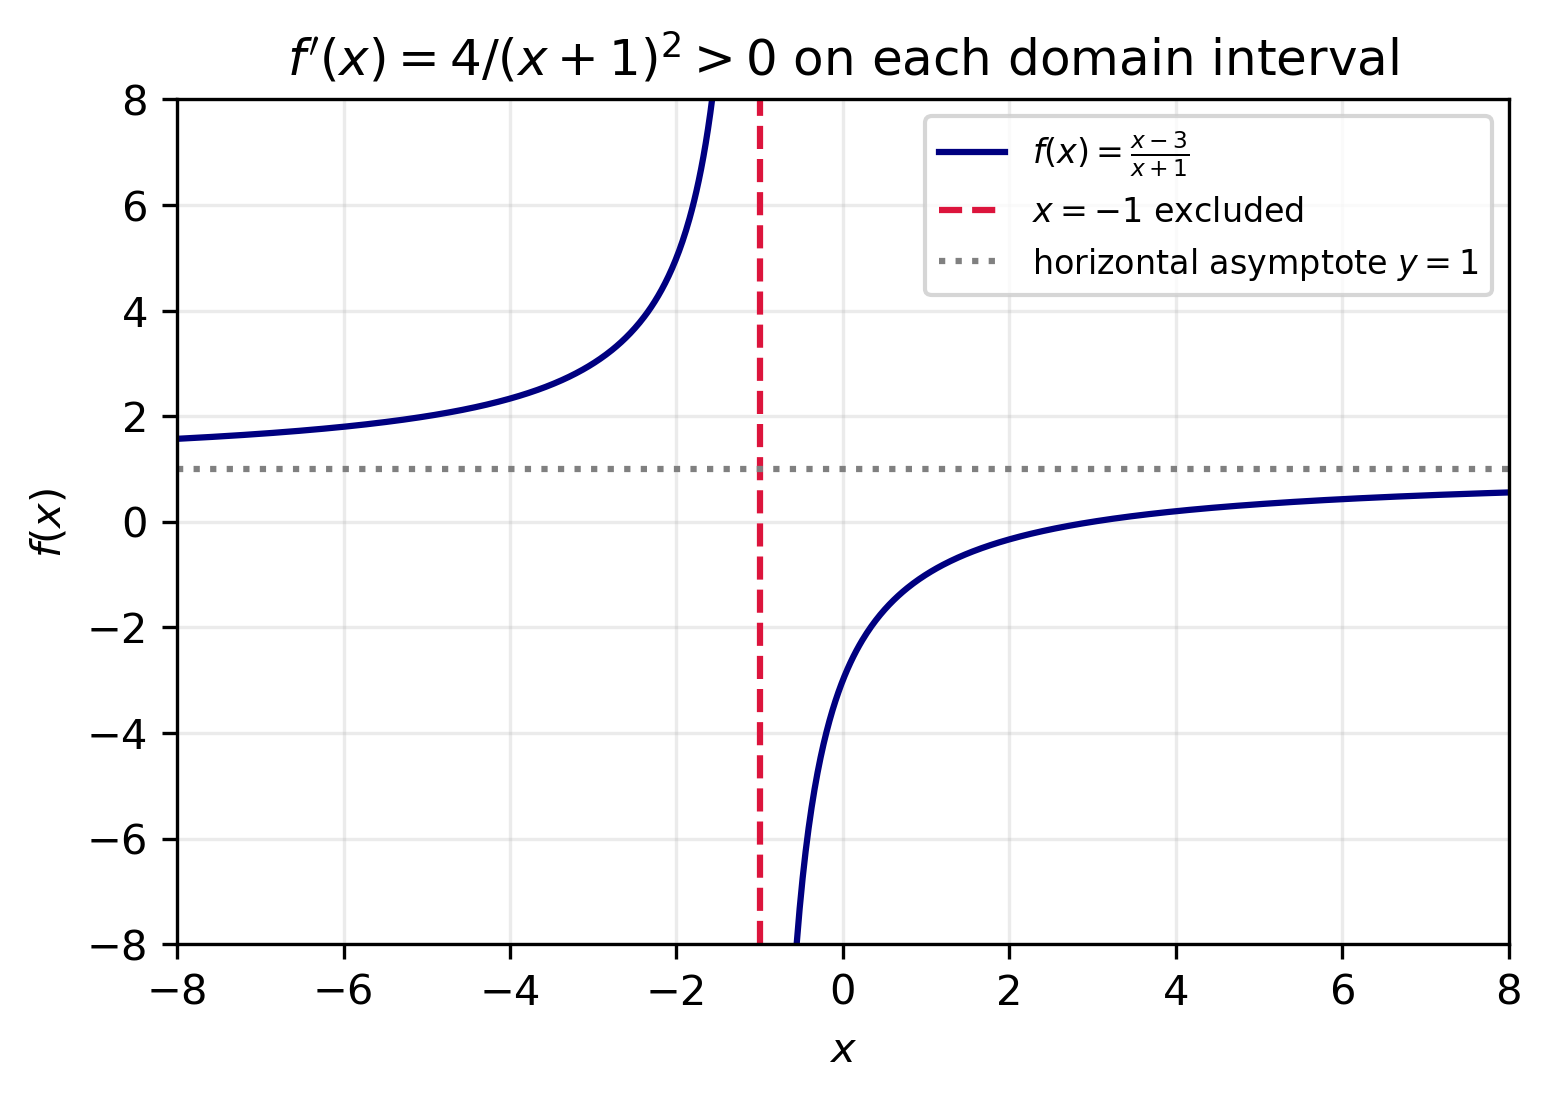
\includegraphics[width=0.51\linewidth]{figs/5.1.23.png}
\caption{The rational function increases on each interval of its domain.}
\end{figure}

\item[5.1.24.1] Three bees fly along vectors $\vec a=2\hat i-3\hat j+\hat k$, $\vec b=4\hat j-2\hat k$, and $\vec c=3\hat i+2\hat k$. Find $\lambda$ such that $\vec a+\lambda\vec b$ is perpendicular to $\vec c$.

\vspace{0.6em}\par\noindent\textbf{Solution:}

Perpendicularity requires $(\vec a+\lambda\vec b)\cdot\vec c=0$. Since $\vec a\cdot\vec c=8$ and $\vec b\cdot\vec c=-4$, we get $8-4\lambda=0$, hence $\boxed{\lambda=2}$.

\item[5.1.24.2] For non-collinear points $A,B,C$, $\overrightarrow{AB}=\hat i+2\hat j-\hat k$ and $\overrightarrow{AC}=2\hat i-3\hat j$. Find the area of $\triangle ABC$.

\vspace{0.6em}\par\noindent\textbf{Solution:}

The area is $\frac12|\overrightarrow{AB}\times\overrightarrow{AC}|$. Their cross product is $(-3,-2,-7)$, whose magnitude is $\sqrt{62}$. Therefore the area is $\boxed{\frac{\sqrt{62}}2}$ square units. The code plots the triangle in 3D and evaluates the cross product.
\begin{lstlisting}[frame=single, basicstyle=\rmfamily, escapeinside={(*@}{@*)}]
(*@\makebox[\dimexpr\linewidth-2\fboxsep-2\fboxrule\relax][c]{codes/5.1.24.2.py}@*)
\end{lstlisting}
\begin{figure}[H]
\centering
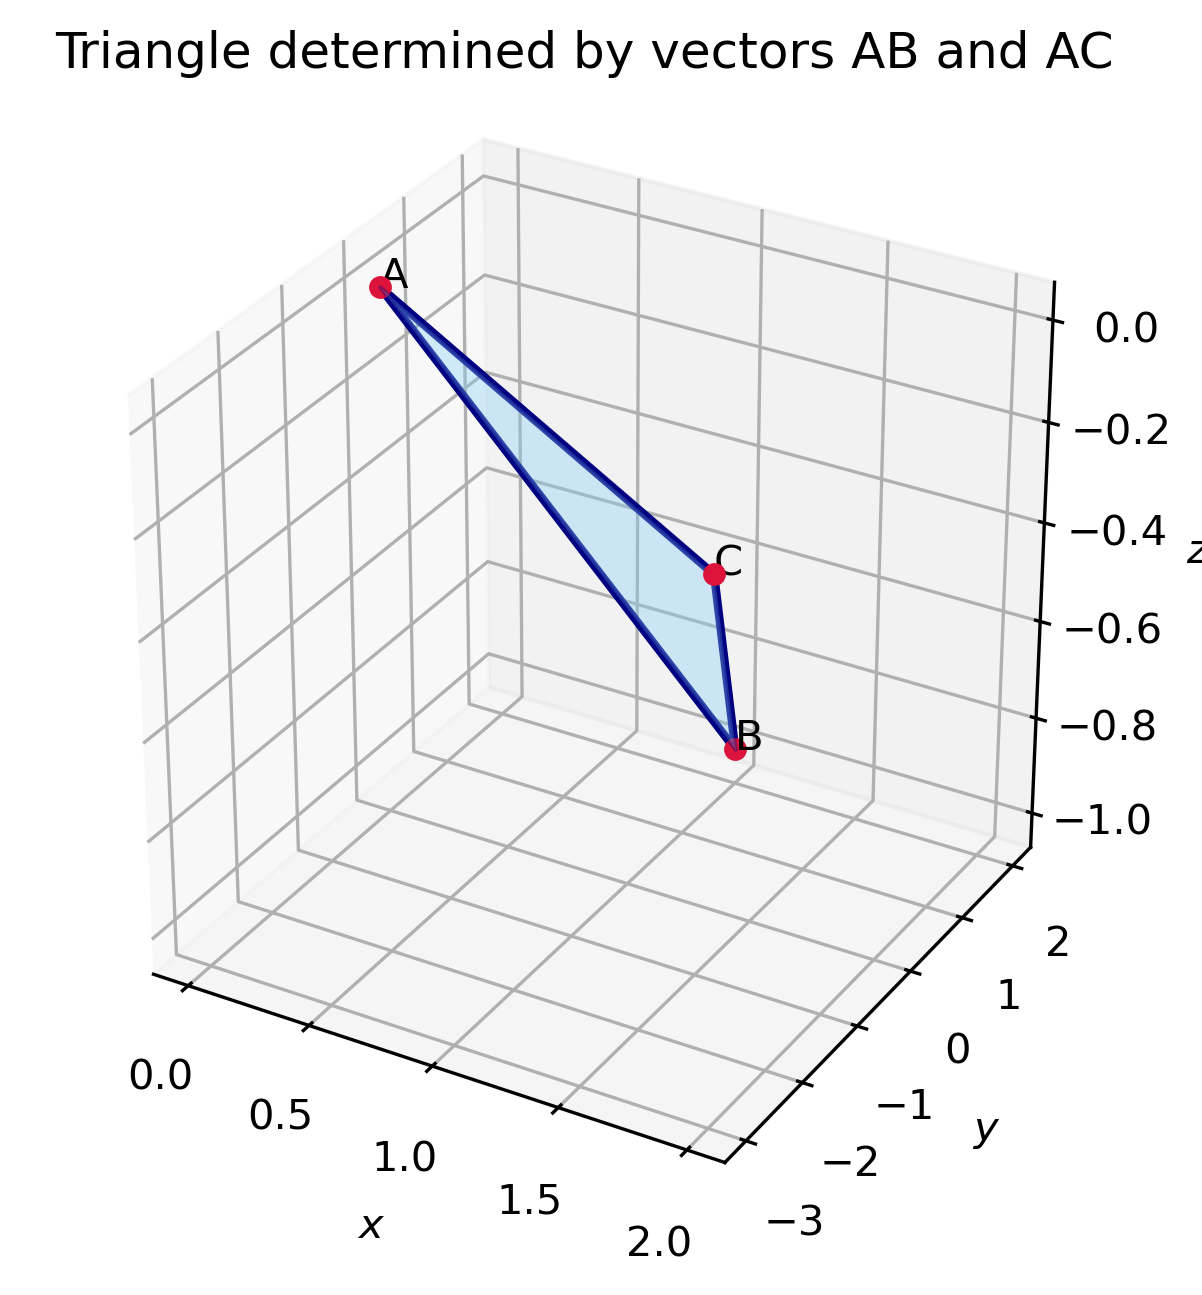
\includegraphics[width=0.48\linewidth]{figs/5.1.24.2.png}
\caption{Triangle formed by the two position-difference vectors.}
\end{figure}

\item[5.1.25] Find the angle between the lines $\frac{x-2}{3}=\frac{y+5}{2}=\frac{1-z}{-6}$ and $\frac{x-7}{1}=\frac{y}{2}=\frac{6-z}{-2}$.

\vspace{0.6em}\par\noindent\textbf{Solution:}

Direction vectors are $(3,2,6)$ and $(1,2,2)$. Their dot product is $19$ and their magnitudes are $7$ and $3$. Thus the acute angle is $\theta=\cos^{-1}(19/21)\approx25.2^\circ$. The code plots both 3D lines and calculates the angle using their direction vectors.
\begin{lstlisting}[frame=single, basicstyle=\rmfamily, escapeinside={(*@}{@*)}]
(*@\makebox[\dimexpr\linewidth-2\fboxsep-2\fboxrule\relax][c]{codes/5.1.25.py}@*)
\end{lstlisting}
\begin{figure}[H]
\centering
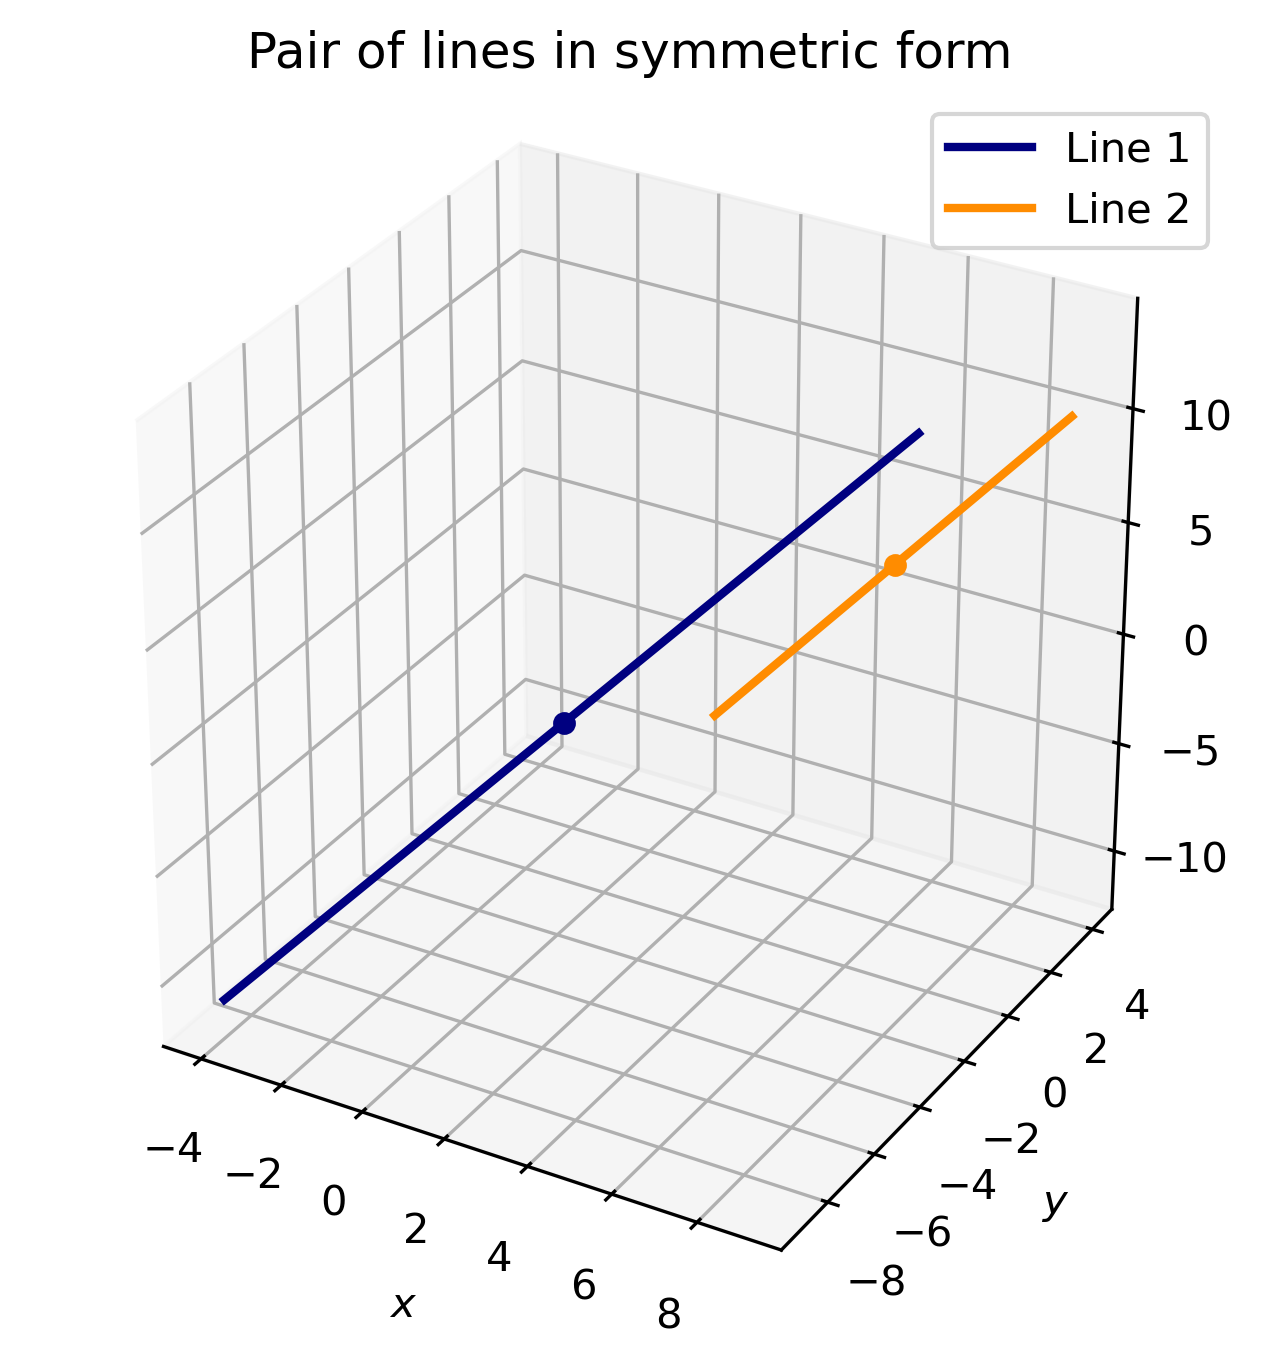
\includegraphics[width=0.48\linewidth]{figs/5.1.25.png}
\caption{The two lines in three-dimensional space.}
\end{figure}

\item[5.1.28] Solve the differential equation $(x+2y^3)\,dy=y\,dx$.

\vspace{0.6em}\par\noindent\textbf{Solution:}

Treat $x$ as a function of $y$: $\frac{dx}{dy}-\frac{x}{y}=2y^2$. The integrating factor is $1/y$, so $\frac{d}{dy}(x/y)=2y$. Integration gives $x/y=y^2+C$, or $\boxed{x=y^3+Cy}$.

\item[5.1.30.2] If $\vec a,\vec b,\vec c$ are unit vectors, prove $|\vec a-\vec b|^2+|\vec b-\vec c|^2+|\vec c-\vec a|^2\le9$.

\vspace{0.6em}\par\noindent\textbf{Solution:}

Using $|\vec a|=|\vec b|=|\vec c|=1$,
\[
|\vec a-\vec b|^2+|\vec b-\vec c|^2+|\vec c-\vec a|^2
=9-|\vec a+\vec b+\vec c|^2\le9.
\]
Equality is possible when the vectors sum to zero, for example when three coplanar unit vectors are $120^\circ$ apart.

\item[5.1.31.1] A die is rolled with $A=\{1,2,5\}$, $B=\{3,5\}$ and $C=\{2,3,4,5\}$. Find (i) $P(A\mid C)$ and $P(C\mid A)$; (ii) $P(A\cap B\mid C)$ and $P(A\cup B\mid C)$.

\vspace{0.6em}\par\noindent\textbf{Solution:}

$A\cap C=\{2,5\}$ and $C\cap A=\{2,5\}$, so $P(A\mid C)=2/4=1/2$ and $P(C\mid A)=2/3$. Also $A\cap B\cap C=\{5\}$, giving $P(A\cap B\mid C)=1/4$. Finally $(A\cup B)\cap C=\{2,3,5\}$, so $P(A\cup B\mid C)=3/4$.

\item[5.1.31.2] A box contains cards numbered $1$ to $6$. Two cards are drawn with replacement. Let $A$ be the event that their sum is $10$ and $B$ the event that the first number is not $4$. Find $P(A\cap B)$ and determine whether $A$ and $B$ are independent.

\vspace{0.6em}\par\noindent\textbf{Solution:}

There are $36$ ordered outcomes. $A=\{(4,6),(5,5),(6,4)\}$ and $A\cap B=\{(5,5),(6,4)\}$, so $P(A\cap B)=2/36=1/18$. But $P(A)P(B)=(3/36)(30/36)=5/72\ne1/18$. Thus the events are not independent.

\item[5.1.32] Four apples, three oranges and two bananas cost $\rupee 60$; two apples, four oranges and six bananas cost $\rupee 90$; six apples, two oranges and three bananas cost $\rupee 70$. Find the price of one fruit of each kind using the matrix method.

\vspace{0.6em}\par\noindent\textbf{Solution:}

Let the prices be $a,o,b$. The system is $4a+3o+2b=60$, $2a+4o+6b=90$, $6a+2o+3b=70$. Solving the corresponding matrix equation gives $a=5$, $o=8$, $b=8$. Thus an apple costs $\rupee 5$, an orange $\rupee 8$, and a banana $\rupee 8$.

\item[5.1.33.1] If $y\sqrt{x^2+1}=\log(\sqrt{x^2+1}-x)$, show that $(x^2+1)\frac{dy}{dx}+xy+1=0$.

\vspace{0.6em}\par\noindent\textbf{Solution:}

Differentiate implicitly. The derivative of the right side is $-1/\sqrt{x^2+1}$. The left derivative is $y'\sqrt{x^2+1}+xy/\sqrt{x^2+1}$. Multiplying by $\sqrt{x^2+1}$ gives $(x^2+1)y'+xy=-1$, which is the required result.

\item[5.1.33.2] Find the derivative with respect to $x$ of $x^{\cot x}+\frac{2x^2-3}{2x^2-x+2}$.

\vspace{0.6em}\par\noindent\textbf{Solution:}

Logarithmic differentiation gives $\frac{d}{dx}x^{\cot x}=x^{\cot x}(\frac{\cot x}{x}-\log x\,\csc^2x)$. By the quotient rule, the derivative of the rational term is $\frac{-2x^2+20x-3}{(2x^2-x+2)^2}$. Add these two expressions for the required derivative.

\item[5.1.34] Sketch $\{(x,y):100x^2+25y^2=2500\}$ and find its enclosed area using integration.

\vspace{0.6em}\par\noindent\textbf{Solution:}

The equation is $x^2/25+y^2/100=1$, an ellipse with semi-axes $5$ and $10$. By symmetry, its area is
\[
4\int_0^5 10\sqrt{1-x^2/25}\,dx=50\pi.
\]
The code plots the ellipse and computes the enclosed area.
\begin{lstlisting}[frame=single, basicstyle=\rmfamily, escapeinside={(*@}{@*)}]
(*@\makebox[\dimexpr\linewidth-2\fboxsep-2\fboxrule\relax][c]{codes/5.1.34.py}@*)
\end{lstlisting}
\begin{figure}[H]
\centering
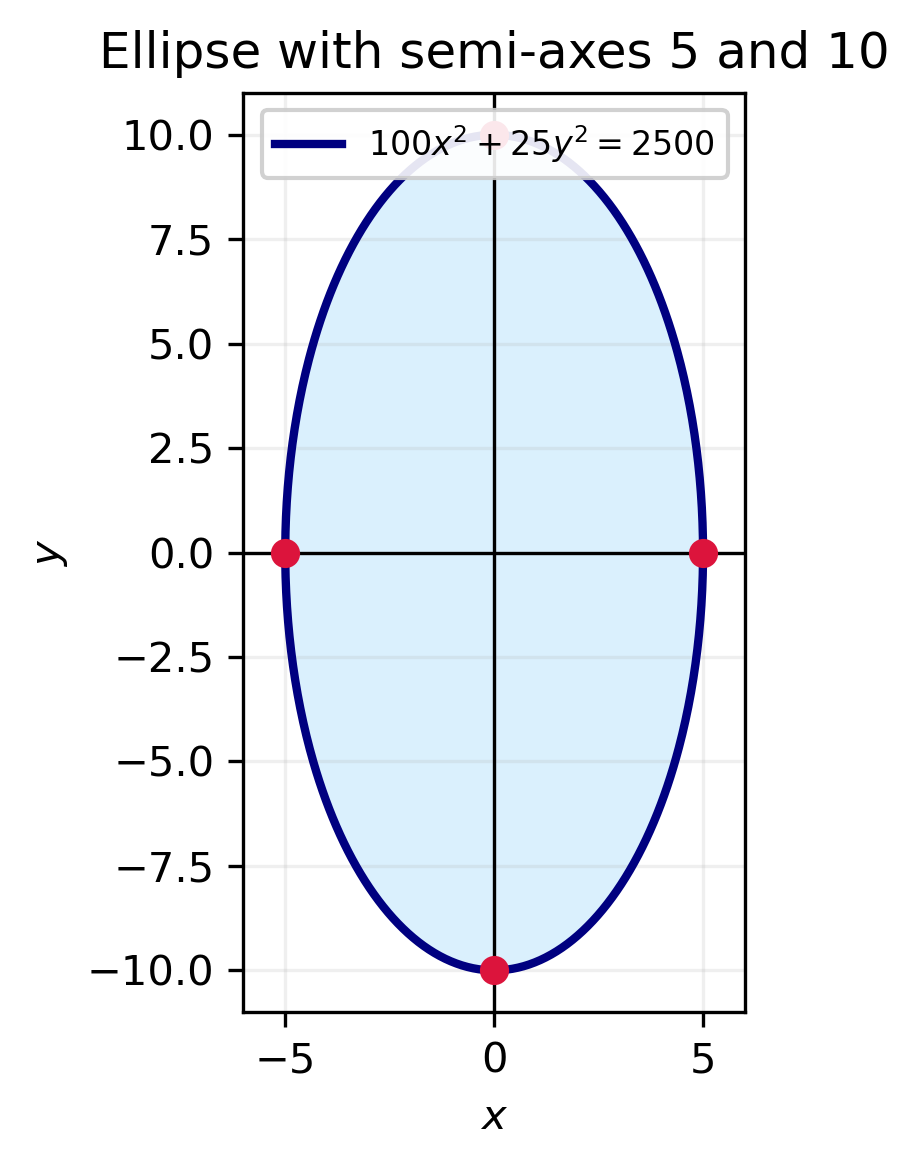
\includegraphics[width=0.49\linewidth]{figs/5.1.34.png}
\caption{Ellipse $x^2/25+y^2/100=1$.}
\end{figure}

\item[5.1.35.1] Find the foot of the perpendicular from $P=(0,2,3)$ to $\frac{-x-3}{-5}=\frac{1-y}{-2}=\frac{3z+12}{9}$ and find its length.

\vspace{0.6em}\par\noindent\textbf{Solution:}

The line passes through $A=(-3,1,-4)$ with direction $\vec d=(5,2,3)$. The projection parameter is $t=\frac{\vec d\cdot(P-A)}{|\vec d|^2}=1$, so the foot is $H=A+\vec d=(2,3,-1)$. Therefore $PH=\sqrt{(-2)^2+(-1)^2+4^2}=\sqrt{21}$. The code plots the line and perpendicular.
\begin{lstlisting}[frame=single, basicstyle=\rmfamily, escapeinside={(*@}{@*)}]
(*@\makebox[\dimexpr\linewidth-2\fboxsep-2\fboxrule\relax][c]{codes/5.1.35.1.py}@*)
\end{lstlisting}
\begin{figure}[H]
\centering
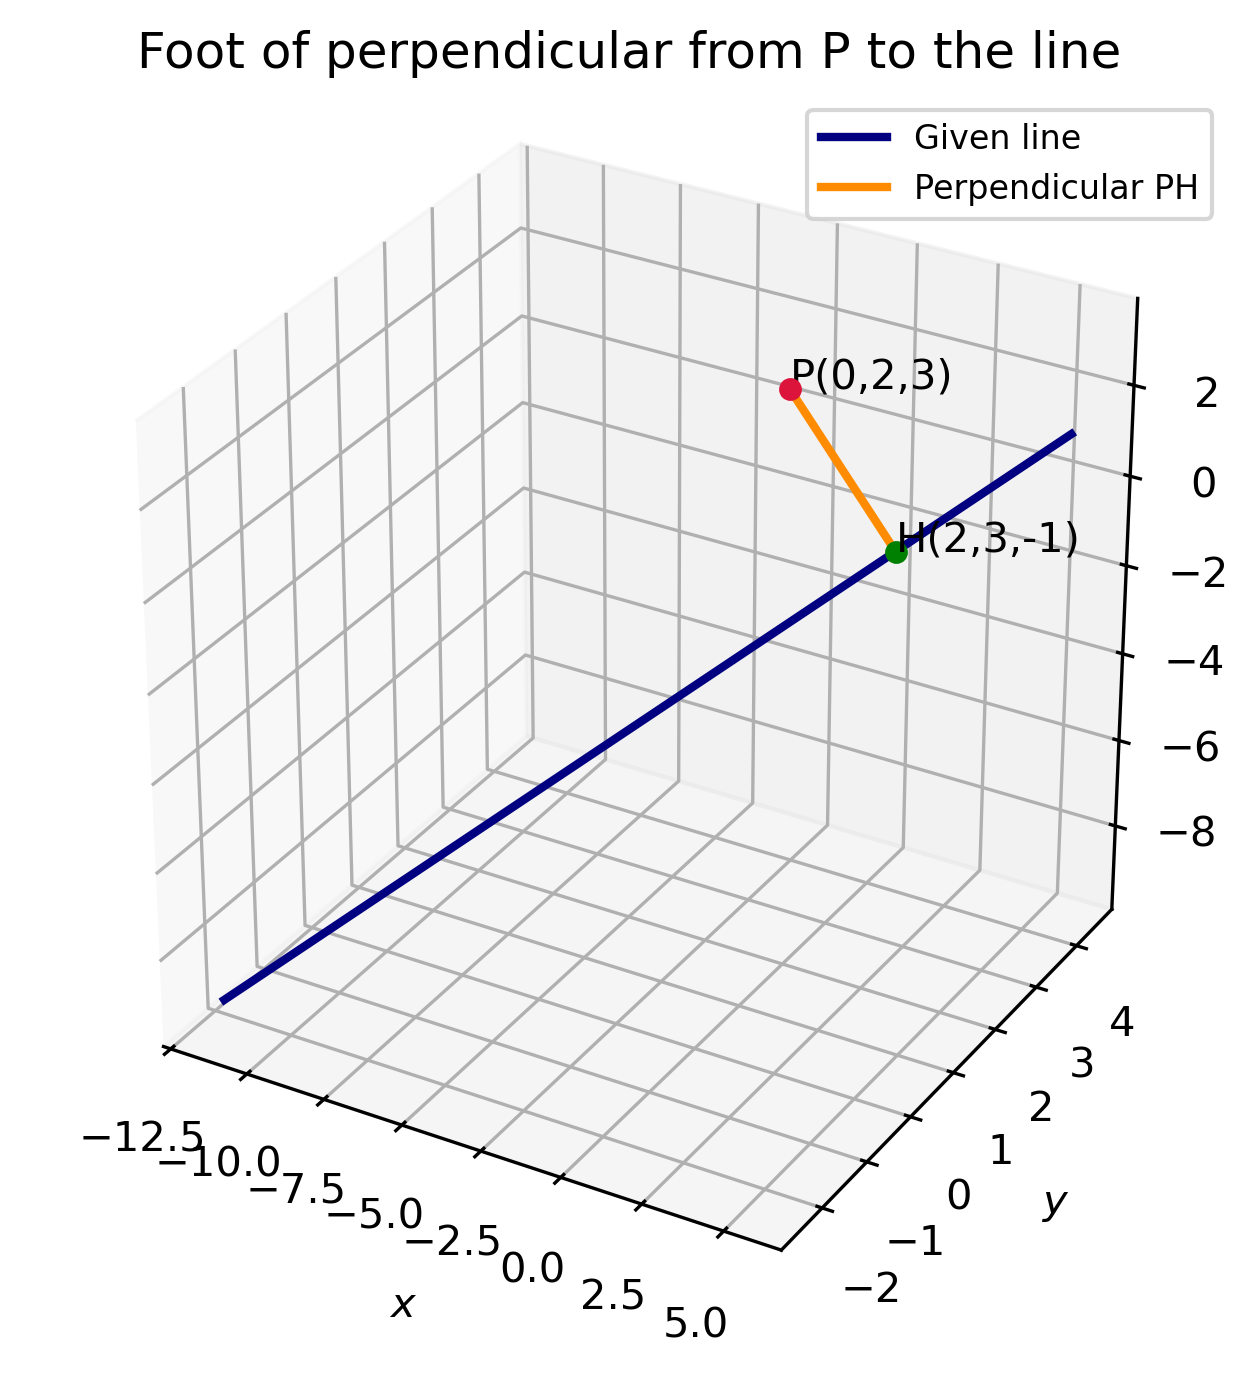
\includegraphics[width=0.48\linewidth]{figs/5.1.35.1.png}
\caption{Perpendicular from $P$ to the given line.}
\end{figure}

\item[5.1.35.2] The shortest distance between $\vec r=(\hat i+2\hat j+\hat k)+\lambda(\hat i-\hat j+\hat k)$ and $\vec r=(p\hat i-\hat j-\hat k)+\mu(2\hat i+\hat j+2\hat k)$ is $3/\sqrt2$. Find $p$.

\vspace{0.6em}\par\noindent\textbf{Solution:}

The direction vectors have cross product $(-3,0,3)$. The skew-line distance is $\frac{|(Q-P)\cdot(\vec d_1\times\vec d_2)|}{|\vec d_1\times\vec d_2|}=\frac{|p+1|}{\sqrt2}$. Equating this to $3/\sqrt2$ gives $|p+1|=3$, so $\boxed{p=2\text{ or }-4}$. The code plots both configurations and evaluates the distance condition.
\begin{lstlisting}[frame=single, basicstyle=\rmfamily, escapeinside={(*@}{@*)}]
(*@\makebox[\dimexpr\linewidth-2\fboxsep-2\fboxrule\relax][c]{codes/5.1.35.2.py}@*)
\end{lstlisting}
\begin{figure}[H]
\centering
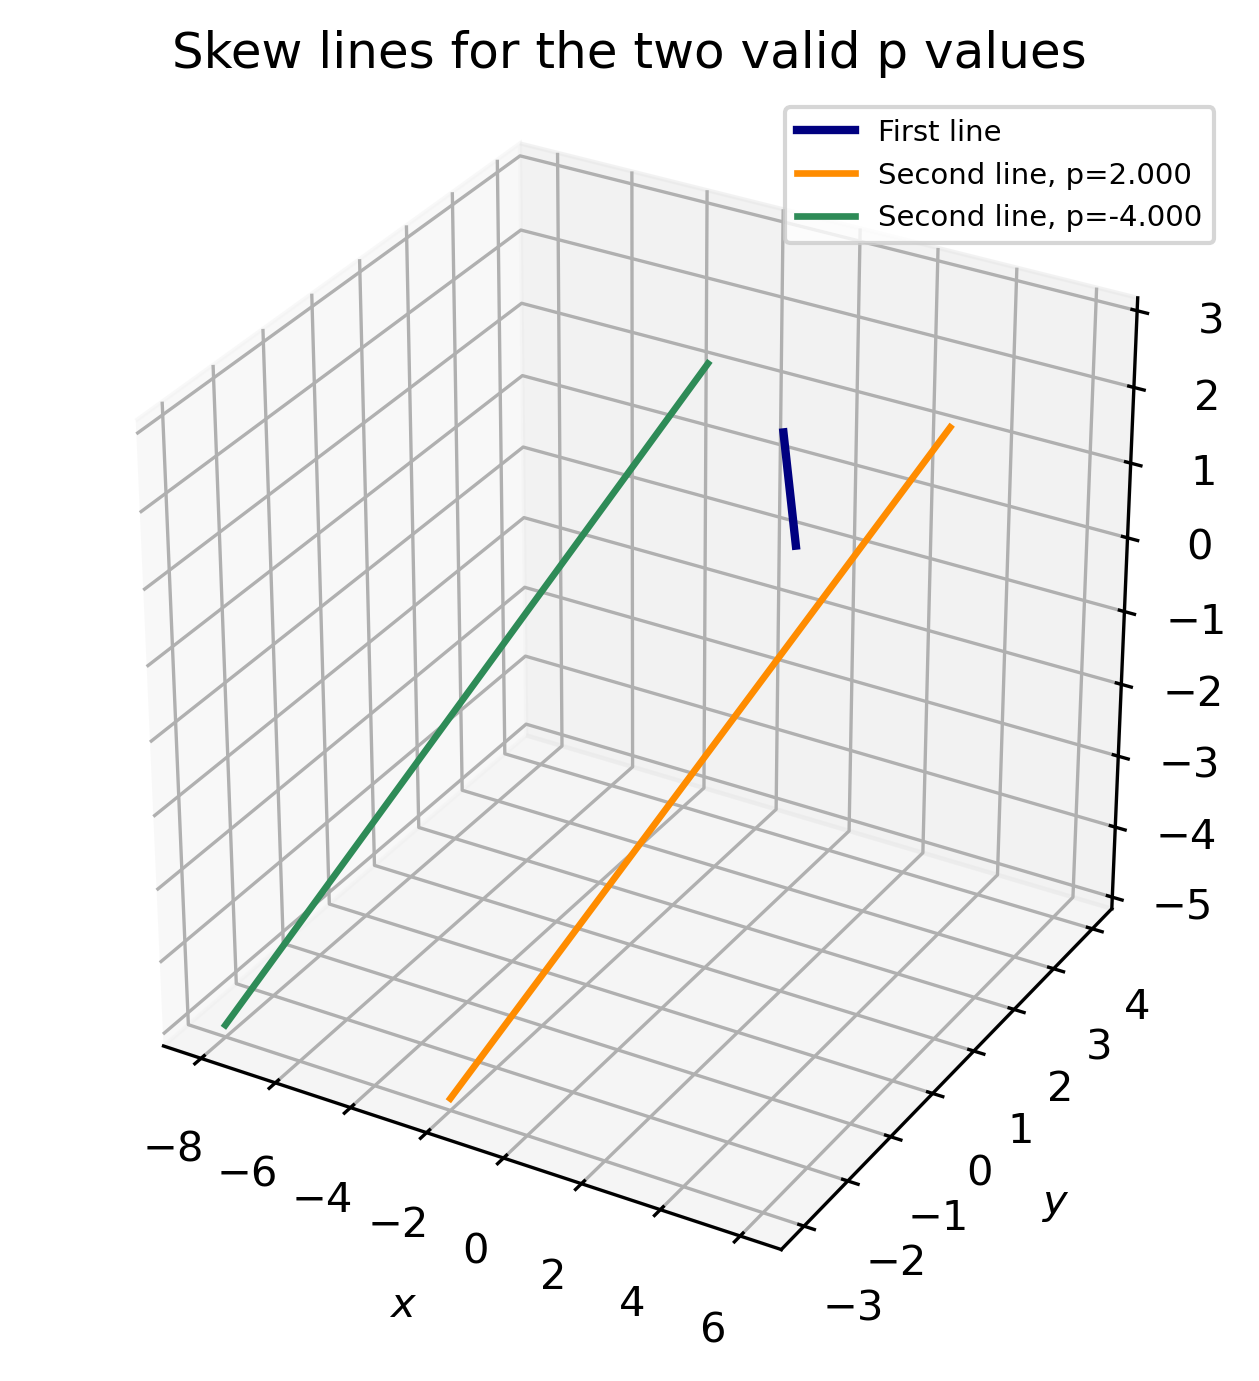
\includegraphics[width=0.48\linewidth]{figs/5.1.35.2.png}
\caption{The skew-line pair for each valid value of $p$.}
\end{figure}

\item[5.1.36] Let $A=\{G_1,G_2,G_3,G_4\}$ and $B=\{B_1,B_2,B_3\}$. Find (i) the number of relations from $A$ to $B$; (ii) whether $R=\{(G_1,B_1),(G_2,B_2),(G_3,B_2),(G_4,B_3),(G_1,B_2)\}$ is an injective function; (iii)(a) whether “students from the same colony” is an equivalence relation, or (iii)(b) whether a bijection $B\to A$ is possible.

\vspace{0.6em}\par\noindent\textbf{Solution:}

There are $2^{4\cdot3}=4096$ relations. In the listed $R$, $G_1$ is paired with two elements, so $R$ is not a function and hence is not an injective function. “Being from the same colony” is reflexive, symmetric and transitive, so it is an equivalence relation. A bijection from $B$ to $A$ is impossible because $|B|=3$ and $|A|=4$. The C program prints these results.
\begin{lstlisting}[frame=single, basicstyle=\rmfamily, escapeinside={(*@}{@*)}]
(*@\makebox[\dimexpr\linewidth-2\fboxsep-2\fboxrule\relax][c]{codes/5.1.36.c}@*)
\end{lstlisting}

\item[5.1.37] Vaccines $A_1,A_2,A_3$ are given to $25\%,35\%,40\%$ of the population. Their respective protection probabilities are $60\%,55\%,50\%$. Find (i) the probability an $A_2$ recipient gets infected; (ii) the probability a randomly chosen person is protected; (iii)(a) the probability an infected person had $A_1$, or (iii)(b) the probability an uninfected person had $A_3$.

\vspace{0.6em}\par\noindent\textbf{Solution:}

(i) $P(I\mid A_2)=1-0.55=0.45$. (ii) $P(P)=0.25(0.60)+0.35(0.55)+0.40(0.50)=0.5425=217/400$, so $P(I)=183/400$.

(iii)(a) $P(A_1\mid I)=\frac{0.25(0.40)}{0.4575}=40/183$. (iii)(b) $P(A_3\mid P)=\frac{0.40(0.50)}{0.5425}=80/217$.
\end{list}

\end{document}
